
%(BEGIN_QUESTION)
% Copyright 2006, Tony R. Kuphaldt, released under the Creative Commons Attribution License (v 1.0)
% This means you may do almost anything with this work of mine, so long as you give me proper credit

Examine the following toroidal conductivity analyzer circuit, then answer the questions that follow:

$$\includegraphics[width=15.5cm]{i04305x01.eps}$$

\begin{itemize}
\item{} If $V_{excitation}$ were to increase, would the millivoltmeter's reading {\it increase}, {\it decrease}, or {\it stay the same}?
\vskip 5pt
\item{} If the conductivity of the liquid were to increase, would the millivoltmeter's reading {\it increase}, {\it decrease}, or {\it stay the same}?
\vskip 5pt
\item{} If the liquid were to completely drain out of the sample holder, would the millivoltmeter's reading {\it increase}, {\it decrease}, or {\it stay the same}?
\vskip 5pt
\item{} If the sampled liquid is tap water, identify something you could do to the water to increase its conductivity.
\end{itemize}

\underbar{file i04305}
%(END_QUESTION)





%(BEGIN_ANSWER)

\begin{itemize}
\item{} If $V_{excitation}$ were to increase, the millivoltmeter's reading would {\bf increase}
\vskip 5pt
\item{} If the conductivity of the liquid were to increase, the millivoltmeter's reading would {\bf increase}
\vskip 5pt
\item{} If the liquid were to completely drain out of the sample holder, the millivoltmeter's reading would {\bf decrease} (all the way to zero)
\vskip 5pt
\item{} You could add salt or some other ionic compound to the water to increase its conductivity.  You could also heat the water to a greater temperature.
\end{itemize}

%(END_ANSWER)





%(BEGIN_NOTES)


%INDEX% Measurement, analytical: conductivity

%(END_NOTES)


